\documentclass[11pt]{article}


\usepackage[utf8]{inputenc}
\usepackage[T1]{fontenc}
\usepackage[french]{babel}
\usepackage{newunicodechar}

\usepackage{graphicx}
\usepackage{fullpage}
\usepackage{times}
\usepackage{color}
\usepackage{needspace}
\usepackage{float}
\usepackage{listings}
\PassOptionsToPackage{hyphens}{url}
\usepackage{hyperref}

\begin{document}


\title{ \huge
  Implémentation de Go-Back-N et contrôle de congestion \\
  \Large Projet 1 de Réseaux I \\}

\author{Groupe 6969696969\\DACHY Corentin (131563), JOSSE Thomas (666)}

\date{Année Académique : 2017 - 2018\\
BAC 2 en Sciences Informatiques\\
\vspace{1cm}
Faculté des Sciences, Université de Mons}

\maketitle

\bigskip
\begin{center} \today \end{center}

\newpage

\section{Construction et exécution}
BLABLABLA comment compiler et exécuter


\section{Section 2}
\section{Section 3}
BLABLABLA
\section{Section 4}
Blabla?
\\ \\ Délicieux anniversaire
\begin{figure}[h]
  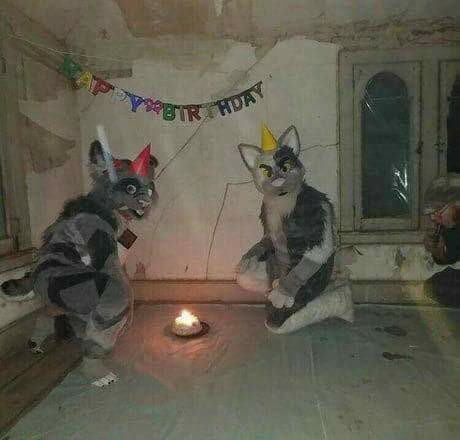
\includegraphics[scale=0.7]{HP.png}
\end{figure}



\end{document}
